\section{Results} \label{sec:results}

\subsection{Franke function}
First we will take a look at how good our linear regression is...
\subsubsection{Visualization of graphes}

 \begin{figure} [H]
 	\centering
 	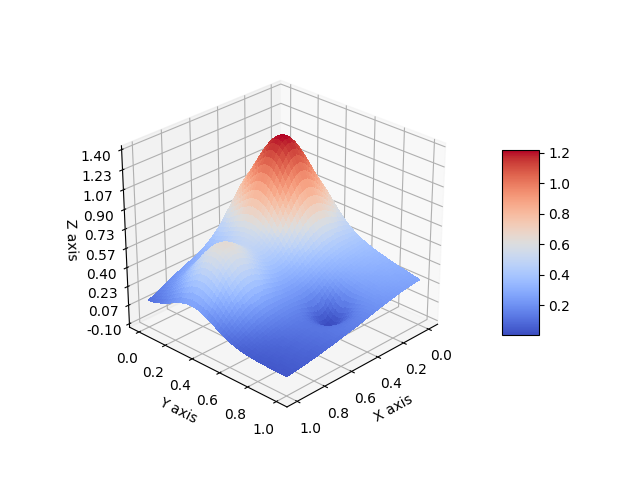
\includegraphics[scale=0.8]{../plots/franke.png}
 	\caption{The Franke function in the interval $x\in[0,1]$, $y\in[0,1]$, $z\in[0, 1.2]$.}
 	\label{fig:franke}
 \end{figure}

 
\newgeometry{left=2cm,right=2cm,top=1cm}
\begin{figure} [H]%
    \centering
    \subfloat[OLS without noise]{{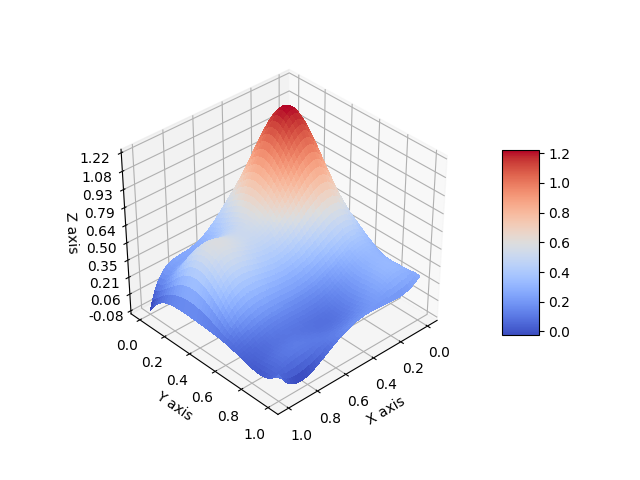
\includegraphics[width=9cm]{../plots/OLS.png} }}%
    \subfloat[OLS with noise]{{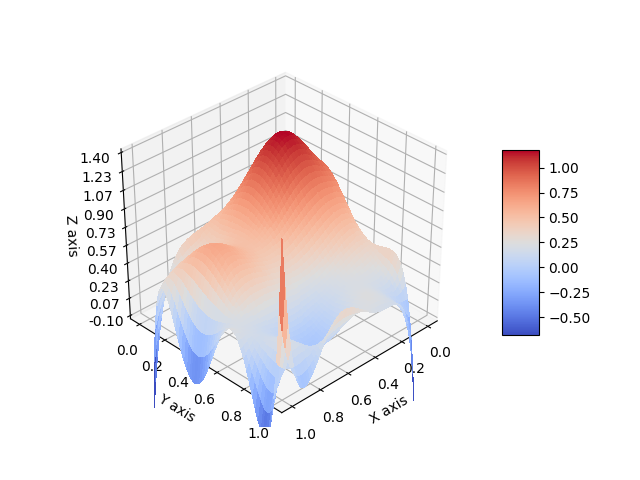
\includegraphics[width=9cm]{../plots/OLS_noise.png} }}\\

    \subfloat[Ridge without noise]{{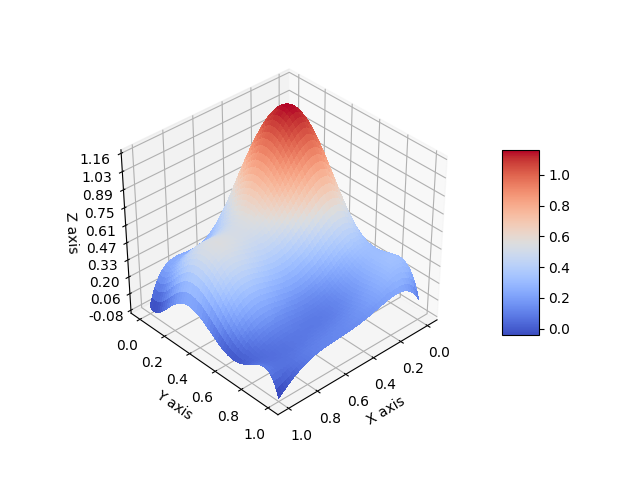
\includegraphics[width=9cm]{../plots/Ridge.png} }}%
    \subfloat[Ridge with noise]{{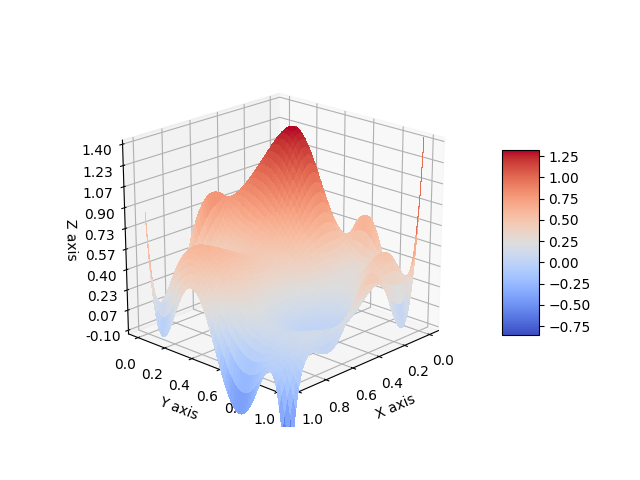
\includegraphics[width=9cm]{../plots/Ridge_noise.png} }}\\
    
    \subfloat[Lasso without noise]{{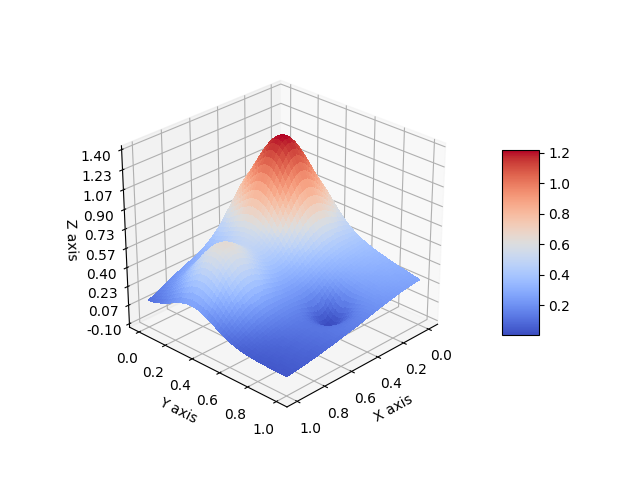
\includegraphics[width=9cm]{../plots/franke.png} }}%
    \subfloat[Lasso with noise]{{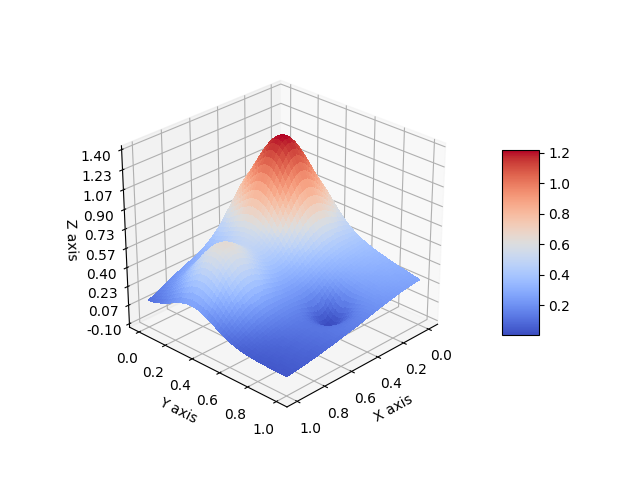
\includegraphics[width=9cm]{../plots/franke.png} }}
    \caption{Fitted polynomial by OLS, Ridge and Lasso with and without noise. For these plots, we used a low penalty of $\lambda=1e-15$.}%
    \label{fig:example}%
\end{figure}

\restoregeometry

\subsubsection{Error}


\subsection{Real data}
First we will take a look at how good our linear regression is...
\subsubsection{Visualization of graphes}

 \begin{figure} [H]
 	\centering
 	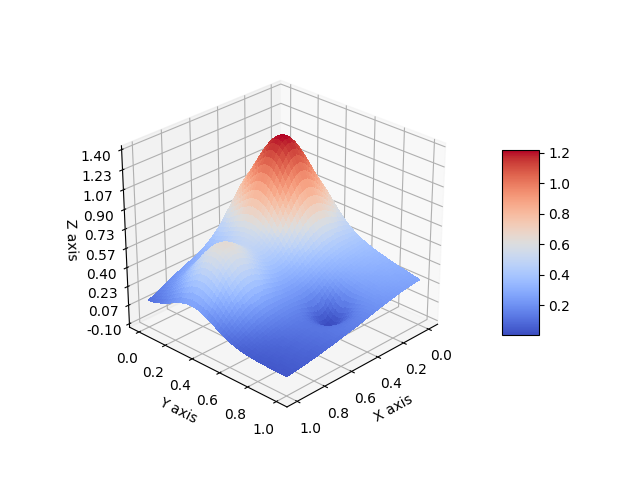
\includegraphics[scale=0.8]{../plots/franke.png}
 	\caption{The Franke function in the interval $x\in[0,1]$, $y\in[0,1]$, $z\in[0, 1.2]$.}
 	\label{fig:franke}
 \end{figure}

 
\newgeometry{left=2cm,right=2cm,top=1cm}
\begin{figure} [H]%
    \centering
    \subfloat[OLS without noise]{{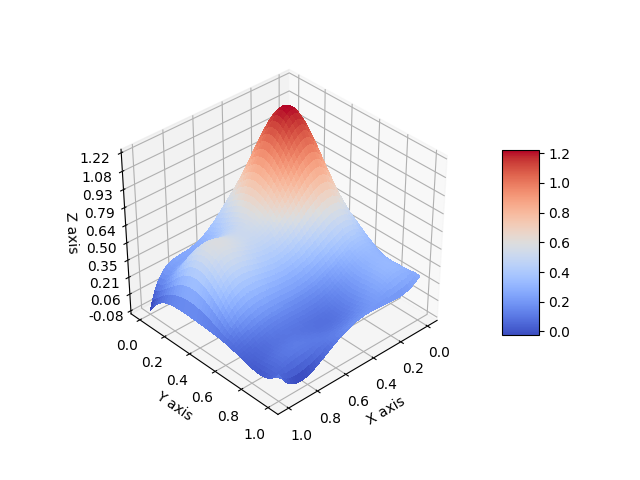
\includegraphics[width=9cm]{../plots/OLS.png} }}%
    \subfloat[OLS with noise]{{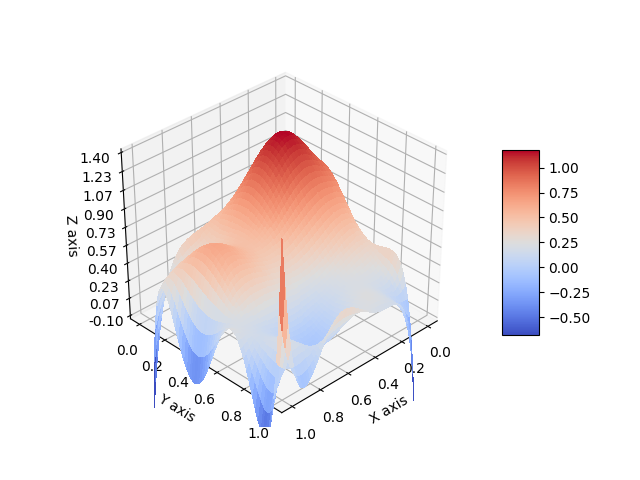
\includegraphics[width=9cm]{../plots/OLS_noise.png} }}\\

    \subfloat[Ridge without noise]{{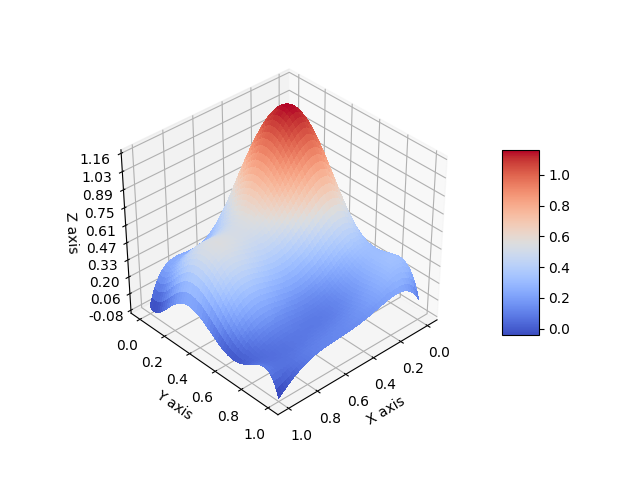
\includegraphics[width=9cm]{../plots/Ridge.png} }}%
    \subfloat[Ridge with noise]{{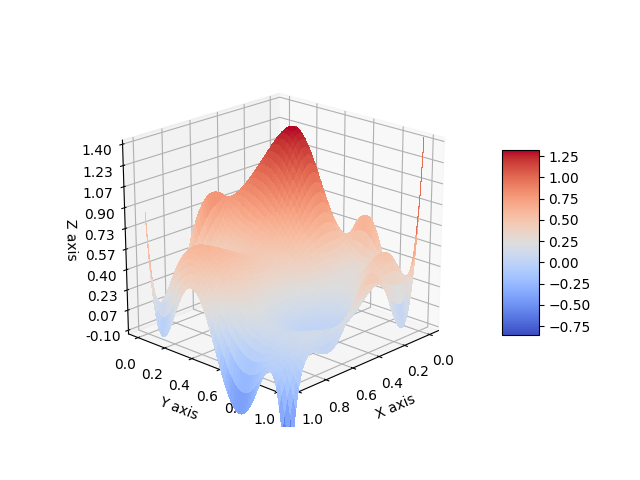
\includegraphics[width=9cm]{../plots/Ridge_noise.png} }}\\
    
    \subfloat[Lasso without noise]{{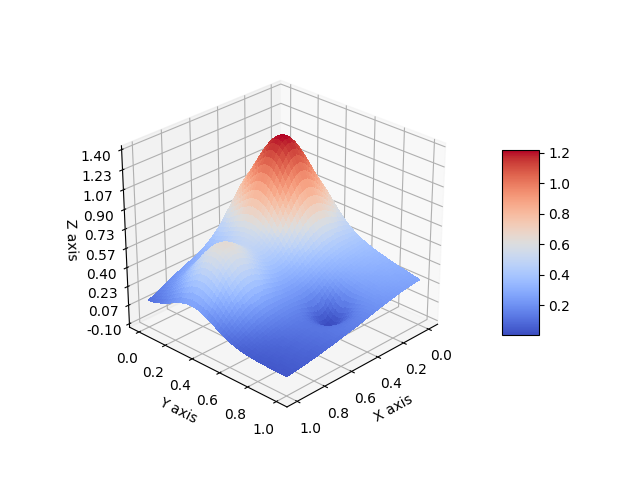
\includegraphics[width=9cm]{../plots/franke.png} }}%
    \subfloat[Lasso with noise]{{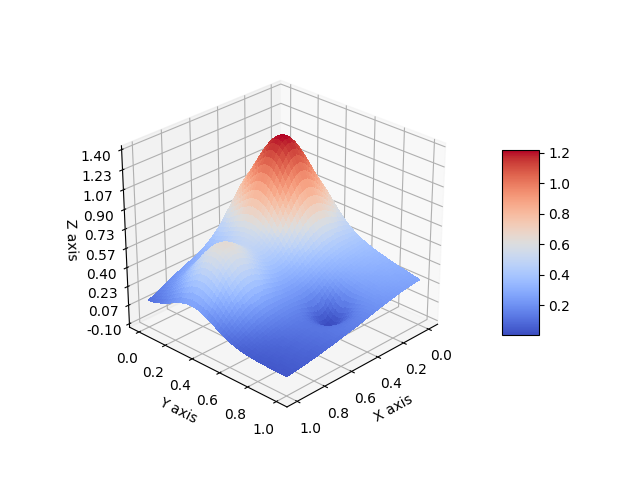
\includegraphics[width=9cm]{../plots/franke.png} }}
    \caption{Fitted polynomial by OLS, Ridge and Lasso with and without noise. For these plots, we used a low penalty of $\lambda=1e-15$.}%
    \label{fig:example}%
\end{figure}



